\documentclass[Main]{subfiles}

\begin{document}
\section{Results and Discussion}
This project have ended with the function $miniproject(t\_errors, errorloc)$ in MatLab which runs the Meggitt decoder.
It will return 1 if the messages has been decoded the correct code word otherwise 0.
It takes the parameters $t\_errors$, which is the number of errors which should be added to the message and $errorloc$ which is the location of the errors.
If $errorloc$ is not used the error is added randomly.

Some screen dumps form MatLab calling the $miniproject()$ function will be discussed.
The result form calling the function with indicating one error is shown in Figure \ref{fig:result-1-errors}.
It can be seen that the codeword has been decoded successfully.
Furthermore it shows the interested vectors and the tag telling what decoding it has done. 

\begin{figure}[h!]
\centering
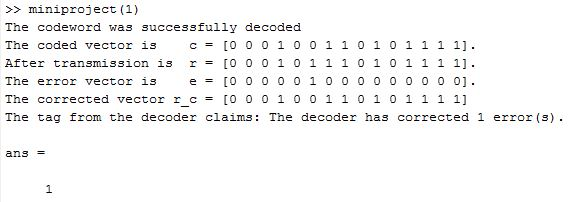
\includegraphics[width=0.7\linewidth]{./Picture/result-1-errors}
\caption{Meggitt decode run with one error, no location}
\label{fig:result-1-errors}
\end{figure}

The Figures \ref{fig:result-2-errors}, \ref{fig:result-2-errors-location} and \ref{fig:result-3-errors} shows the result with other inputs.
In Figure \ref{fig:result-3-errors} it is seen that it is possible to detect there is more errors than 2 but it is not able to correct it. 

\begin{figure}[h!]
\centering
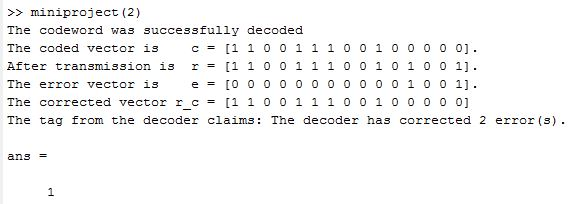
\includegraphics[width=0.7\linewidth]{./Picture/result-2-errors}
\caption{Meggitt decoder run with two errors, no location}
\label{fig:result-2-errors}
\end{figure}

\begin{figure}[h!]
\centering
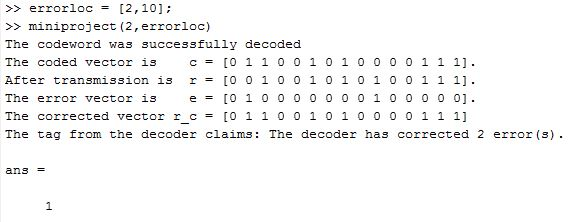
\includegraphics[width=0.7\linewidth]{./Picture/result-2-errors-location}
\caption{Meggit decoder run with 2 errors, with location}
\label{fig:result-2-errors-location}
\end{figure}

\begin{figure}[h!]
\centering
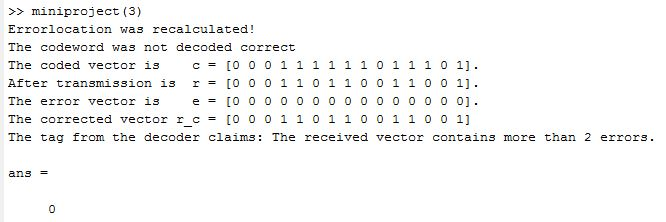
\includegraphics[width=0.7\linewidth]{./Picture/result-3-errors}
\caption{Meggitt decoder run with 3 errors, no location}
\label{fig:result-3-errors}
\end{figure}

Simultaneous with the code development, all the steps have been calculated by hand as well.
The calculation in hand has worked as an secure that the program has been developed in the right way.
A codeword has been generated and tested in MatLab and by hand and the result have been match.
When the result was different the procedure has been check and errors have been corrected.

The function $miniproject(t\_errors, errorloc)$ is able to correct 1 and 2 errors on a codeword, which can be seen in Figure \ref{fig:result-1-errors}, \ref{fig:result-2-errors} and \ref{fig:result-2-errors-location}.
It is also possible to detect more errors.
So when sending in 3 errors it is not possible to correct them but it is able to detect that there is more than 2 errors, see Figure \ref{fig:result-3-errors}.\\
It is possible to sending an codeword with 3 errors which is able to correct to at valid codeword.
At first this gave some frustration until putting some bit deeper thought into this.
A possible cause to this could be that when adding 3 errors to a codeword can result in a codeword with only 2 errors, which the function is able to correct to a valid codeword.
A bit more explanations is here:
The general polynomial has a weight of 5 which give a $d_{min}=5$.
When only adding 2 or less errors it is sure that the shortest distance is to the correct codeword.
When adding 3 or more, there is at possibility that it is getting a distance of two to an other codeword.
In the way the $miniproject(t\_errors, errorloc)$ has been implemented it will always look for the codeword with the shortest distance which it is why it will reach a valid but wrong codeword.
This might be corrected in the code so when 1 error has been found it know that is there should be another error it should be when there is only one error in the rightmost bit.
So by minimising the error pattern table when an error has been detected insure that the function don't use the error pattern for 2 error twice.
This is not implemented in MatLab, but would be a next step to go. 



\end{document}
